\documentclass[a4paper,12pt]{article}

\usepackage{mystyle}

\graphicspath{ {images/} }


\author{Алексеев Василий}
\title{Семинар 4}
\date{22 + 28 сентября 2020}


\begin{document}
  \maketitle
  
  \tableofcontents

  \thispagestyle{empty}
  
  \newpage
  
  \pagenumbering{arabic}


  \section{Смешанное и векторное произведения}
  
  \subsection{Ориентированное пространство}
  
  \begin{figure}[h]
    \centering
    
    \includegraphics[width=0.8\columnwidth]{two-classes}
    
    \caption{Разные классы базисов в одно-, дву- и трёхмерном пространствах.}
    \label{fig:two-classes}
  \end{figure}
  
  На прямой все векторы делятся на два класса: направленные в одну сторону вдоль прямой и в противоположную (\ref{fig:two-classes}).
  На плоскости все упорядоченные пары неколлинеарных векторов делятся на два класса: пары, где поворот от первого вектора ко второму по наименьшему углу совершается против часовой стрелки, и пары, где этот поворот совершается по часовой стрелке (\ref{fig:two-classes}).
  И в трёхмерном пространстве все упорядоченные тройки некомпланарных векторов делятся на два класса: те, где поворот от первого базисного вектора ко второму по наименьшему углу происходит против часовой стрелки, если смотреть со стороны третьего базисного вектора (\emph{правые} базисы), и те, где этот поворот происходит по часовой стрелке (\emph{левые} базисы) (\ref{fig:two-classes}).
  
  \begin{definition}
    Ориентированное пространство~---~пространство, в котором выбран класс базисов\footnote{В общем случае пространства $\RR^n$, $n \hm\geq 1$ базисы тоже образуют два класса.}.
  \end{definition}
  
  В ориентированном пространстве можно говорить о длине, площади и объёме со знаком.
  
  \begin{figure}[h]
    \centering
    
    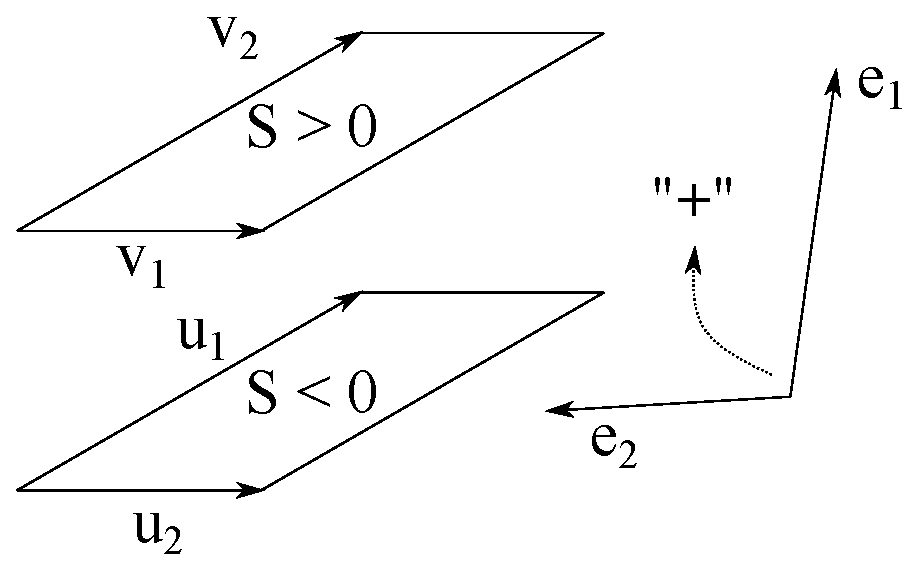
\includegraphics[width=0.5\columnwidth]{two-parallelograms}
    
    \caption{Площадь ориентированного параллелограмма.}
    \label{fig:two-parallelograms}
  \end{figure}
  
  Так, в одномерном пространстве, если рассматриваемый вектор направлен так же, как и базисы в выбранном классе, то его длина считается большей нуля.
  В противном случае~---~меньше нуля.
  В двумерном пространстве, если параллелограмм построен на \emph{упорядоченной} паре векторов $\bds a$ и $\bds b$, то его площадь со знаком $S_{\pm}$ можно считать большей нуля, если $\bds a$ и $\bds b$ образуют базис, относящийся к выбранному (положительному) классу (\ref{fig:two-parallelograms}).
  Иначе~---~меньше нуля.
  И в трёхмерном пространстве, если параллелепипед построен на \emph{упорядоченной} тройке векторов $\bds a$, $\bds b$, $\bds c$, которые в таком же порядке образуют базис из выбранного (положительного) класса, то объём со знаком $V_{\pm}$ такого параллелепипеда будет больше нуля.
  Иначе, если тройка $\bds a$, $\bds b$, $\bds c$ не принадлежит положительному классу базисов, то объём $V_{\pm}$ параллелепипеда будет меньше нуля.
  
  \emph{В трёхмерном пространстве положительными выбраны правые базисы.}
  
  Упомянув трёхмерное пространство, стоит ещё раз вернуться к вопросу об ориентации плоскости.
  Выбор ориентации в $3$D ничего не говорит об ориентации на конкретной плоскости.
  Задать ориентацию на плоскости можно
  \begin{itemize}
    \item В $2$D~---~просто сказав, в какую сторону поворот от $\bds e_1$ к $\bds e_2$ по наименьшему углу считается положительным.
    
    \item В $3$D~---~выбрав вектор нормали $\bds n$ к плоскости.
    Тогда положительный базис на плоскости~---~тот, который с выбранной нормалью составляет положительную тройку в пространстве (порядок $\bds e_1$, $\bds e_2$, $\bds n$ или $\bds n$, $\bds e_1$, $\bds e_2$~---~не важно).
    
    \item Как в $2$D, так и в $3$D: просто выбрав упорядоченную пару неколлинеарных векторов и сказав, что этот базис положительный (тогда и все упорядоченные пары векторов из этого же класса~---~тоже положительные).
  \end{itemize}

  
  \subsection{Смешанное произведение}
  
  \begin{definition}
    В ориентированном пространстве смешанное произведение трёх некомпланарных векторов $\bds a$, $\bds b$, $\bds c$ полагается равным объёму ориентированного параллелепипеда, построенного на векторах $\bds a$, $\bds b$, $\bds c$:
    \[
      (\bds a, \bds b, \bds c) \equiv V_{\pm}(\bds a, \bds b, \bds c)
    \]
    
    Если вектора $\bds a$, $\bds b$, $\bds c$ компланарны, то их смешанное произведение полагается равным нулю.
  \end{definition}
  
  \begin{theorem}[О связи смешанного и скалярного произведения]
    Для любой пары векторов $\bds b$, $\bds c$ существует единственный вектор $\bds d$, такой что для любого вектора $\bds a$
    \[
      (\bds a, \bds b, \bds c) = (\bds a, \bds d)
    \]
  \end{theorem}
  
  \begin{proof}
    Найдём такой вектор $\bds d$ для произвольной тройки векторов $\bds a$, $\bds b$, $\bds c$ и покажем, что он единственен и не зависит от $\bds a$.
    
    Пусть $\bds b$, $\bds c$ неколлинеарны.
    Пусть также $\bds a$, $\bds b$ и $\bds c$ некомпланарны.
    Отложим вектора $\bds a$, $\bds b$, $\bds c$ от одной точки (\ref{fig:triple-product}).
    
    \begin{figure}[h]
      \centering
      
      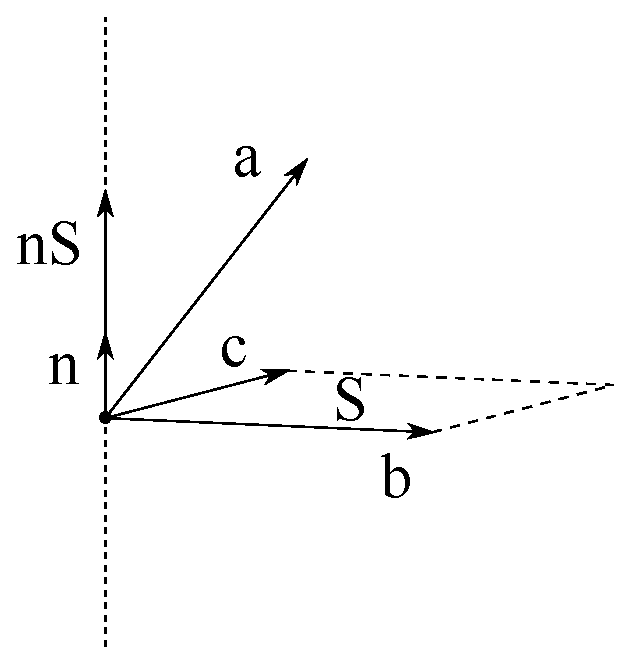
\includegraphics[width=0.5\columnwidth]{triple-product}
      
      \caption{Некомпланарные векторы $\bds a$, $\bds b$, $\bds c$; единичный вектор нормали $\bds n$ к плоскости векторов $\bds b$ и $\bds c$, такой что тройка $\bds b$, $\bds c$, $\bds n$ положительная; $S$~---~площадь параллелограмма, построенного на $\bds b$ и $\bds c$.}
      \label{fig:triple-product}
    \end{figure}
  
    Рассмотрим пару векторов $\bds b$, $\bds c$.
    Отложим единичный вектор нормали $\bds n$ к плоскости векторов $\bds b$, $\bds c$ так, чтобы тройка векторов $\bds b$, $\bds c$, $\bds n$ была бы положительной.
    Площадь параллелограмма, построенного на векторах $\bds b$ и $\bds c$ (площадь без знака) равна
    \[
      S = |\bds b| \cdot |\bds c| \cdot \sin\alpha
    \]
    где $\alpha$~---~угол между векторами $\bds b$ и $\bds c$.
    Тогда $\bds d \hm\equiv S \hm\cdot \bds n$~---~вектор, направленный вдоль $\bds n$ и по модулю равный площади основания параллелепипеда, где лежат вектора $\bds b$, $\bds c$.
    При этом можно заметить, что скалярное произведение
    \[
      (\bds a, \bds d) = V_{\pm}(\bds a, \bds b, \bds c)
    \]
    так как $|(\bds a, \bds d)| \hm= |V_{\pm}|$ (площадь параллелепипеда равна произведению площади основания на высоту, проведённую к этому основанию) и от того, сонаправлены или противоположно направлены вектора $\bds a$ и $
    \bds d$, зависит, будет ли $V_{\pm}$ больше нуля или меньше нуля (тройка $\bds a$, $\bds b$, $\bds n$ по построению положительная; тройка $\bds a$, $\bds b$, $\bds c$ может быть как положительной, так и отрицательной).
    Таким образом, получаем, что
    \[
      (\bds a, \bds b, \bds c) = (\bds a, \bds d)
    \]
    
    Если же векторы $\bds a$, $\bds b$ и $\bds c$ компланарны, то объём параллелепипеда будет равен нулю, но тогда и $\bds d \hm\perp \bds a$.
    
    Если же вектора $\bds b$, $\bds c$ коллинеарны, то смешанное произведение $(\bds a, \bds b, \bds c)$ также будет равно нулю, и вектор $\bds d$ можно взять равным нулю.
    
    Покажем, что такой вектор $\bds d$, что $(\bds a, \bds b, \bds c) \hm= (\bds a, \bds d)$, $\forall \bds a$ единственен.
    Допустим противное: пусть существует вектор $\bds d_1$, такой что $(\bds a, \bds b, \bds c) \hm= (\bds a, \bds d)$ и $(\bds a, \bds b, \bds c) \hm= (\bds a, \bds d_1)$, $\forall \bds a$.
    Но тогда $(\bds a, \bds d) \hm= (\bds a, \bds d_1)$, и $(\bds a, \bds d \hm- \bds d_1) \hm= 0$.
    То есть вектор $\bds d \hm- \bds d_1$ перпендикулярен любому вектору пространства.
    Поэтому $\bds d \hm- \bds d_1 \hm= \bds 0 \hm\Rightarrow \bds d \hm= \bds d_1$.
  \end{proof}
  
  Введённый выше вектор $\bds d$ называется векторным произведением векторов $\bds b$ и $\bds c$.
  
  \subsection{Векторное произведение}
  
  \begin{definition}
    Векторным произведением неколлинеарных векторов $\bds b$ и $\bds c$ называется вектор $\bds d$, такой что
    \begin{itemize}
      \item Модуль вектора $\bds d$ равен
      \[
        |\bds d| = |\bds b| \cdot |\bds c| \cdot \sin\alpha
      \]
      где $\alpha$~---~угол между векторами $\bds b$ и $\bds c$.
      
      \item Вектор $\bds d$ перпендикулярен как вектору $\bds b$, так и вектору $\bds c$:
      \[
        \bds d \perp \bds b,\ \bds d \perp \bds c
      \]
      
      \item Вектор $\bds d$ образует \emph{положительную тройку} $(\bds b, \bds c, \bds d)$ вместе с исходными $\bds b$ и $\bds c$\footnote{При выбранной правой ориентации пространства тройка $(\bds b, \bds c, \bds d)$ должна быть правой.}.
    \end{itemize}
    
    Если же векторы $\bds b$ и $\bds c$ коллинеарны, то их векторное произведение полагается равным нулю.
    
    Векторное произведение $\bds b$ и $\bds c$ может обозначаться как $[\bds b, \bds c]$ или $\bds b \hm\times \bds c$.
  \end{definition}
  
  Таким образом,
  \begin{equation}\label{eq:triple-as-scalar-and-vector}
    (\bds a, \bds b, \bds c) = (\bds a, [\bds b, \bds c])
  \end{equation}
  
  Рассмотрим некоторые свойства векторного произведения.
  
  Так, векторное произведение вектора $\bds a$ на самого себя равно нулю, так как $\bds a \hm\parallel \bds a$:
  \[
    [\bds a, \bds a] = \bds 0
  \]
  
  \begin{figure}[h]
    \centering
    
    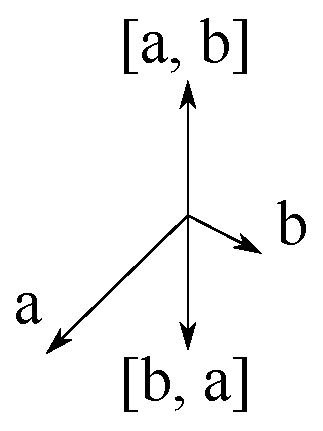
\includegraphics[width=0.25\columnwidth]{ab-ba}
    
    \caption{Векторное произведение антикоммутативно.}
    \label{fig:ab-ba}
  \end{figure}
    
  Для любых $\bds a$ и $\bds b$
  \[
    [\bds a, \bds b] = -[\bds b, \bds a]
  \]
  так как первый и второй вектора меняются местами, и направление поворота от первого вектора ко второму меняется на противоположное (\ref{fig:ab-ba}).
  
  При этом в смешанном произведении сомножители тоже можно переставлять, и, если класс тройки меняется, то меняется и знак перед смешанным произведением:
  \begin{equation}\label{eq:triple-change-order}
    (\bds a, \bds b, \bds c) = -(\bds b, \bds a, \bds c) = \ldots = (\bds c, \bds a, \bds b)
  \end{equation}

  И свойство линейности векторного произведения по первому аргументу:
  \[
    [\beta_1 \bds b_1 + \beta_2 \bds b_2, \bds c] = \beta_1 [\bds b_1, \bds c] + \beta_2 [\bds b_2, \bds c]
  \]
  
  \begin{proof}
    Докажем это свойство.
    Надо ``в нужное время вставлять и убирать квадратные скобки'' и пользоваться линейность скалярного произведения:
    \begin{equation}
    \begin{split}
      (\bds a, [\beta_1 \bds b_1 + \beta_2 \bds b_2, \bds c])
      &\stackrel{(\ref{eq:triple-as-scalar-and-vector})}{=} (\bds a, \beta_1 \bds b_1 + \beta_2 \bds b_2, \bds c)\\
      &\stackrel{(\ref{eq:triple-change-order})}{=}         {-}(\beta_1 \bds b_1 + \beta_2 \bds b_2, \bds a, \bds c)\\
      &\stackrel{(\ref{eq:triple-as-scalar-and-vector})}{=} {-}(\beta_1 \bds b_1 + \beta_2 \bds b_2, [\bds a, \bds c])\\
      &\stackrel{\hphantom{(1)}}{=}                         {-}\beta_1(\bds b_1, [\bds a, \bds c]) - \beta_2(\bds b_2, [\bds a, \bds c])\\
      &\stackrel{(\ref{eq:triple-as-scalar-and-vector})}{=} {-}\beta_1(\bds b_1, \bds a, \bds c) - \beta_2(\bds b_2, \bds a, \bds c)\\
      &\stackrel{(\ref{eq:triple-change-order})}{=}         \beta_1(\bds a, \bds b_1, \bds c) + \beta_2(\bds a, \bds b_2, \bds c)\\
      &\stackrel{(\ref{eq:triple-as-scalar-and-vector})}{=} \beta_1(\bds a, [\bds b_1, \bds c]) + \beta_2(\bds a, [\bds b_2, \bds c])
      \stackrel{\hphantom{(1)}}{=}                         (\bds a, \beta_1[\bds b_1, \bds c] + \beta_2[\bds b_2, \bds c])
    \end{split}
    \end{equation}
  \end{proof}
  
  Теперь можно выразить векторное произведение между произвольными двумя векторами $\bds a$ и $\bds b$ пространства, которые заданы компонентами в некотором базисе $e \hm= (\bds e_1, \bds e_2, \bds e_3)$.
  Пусть
  \[
    \left\{
      \begin{aligned}
        &\bds a = a_1 \cdot \bds e_1 + a_2 \cdot \bds e_2 + a_3 \cdot \bds e_3\\
        &\bds b = b_1 \cdot \bds e_1 + b_2 \cdot \bds e_2 + b_3 \cdot \bds e_3
      \end{aligned}
    \right.
  \]
  Тогда
  \begin{equation*}
  \begin{split}
    \bds a \times \bds b
    =\; &(a_1 \cdot \bds e_1 + a_2 \cdot \bds e_2 + a_3 \cdot \bds e_3) \times (b_1 \cdot \bds e_1 + b_2 \cdot \bds e_2 + b_3 \cdot \bds e_3)\\
    =\; &(a_2 b_3 - a_3 b_2)[\bds e_2, \bds e_3] + (a_1 b_3 - a_3 b_1)[\bds e_1, \bds e_3] + (a_1 b_2 - a_2 b_1)[\bds e_1, \bds e_2]
  \end{split}
  \end{equation*}
  где в последнем переходе использовались свойство антикоммутативности векторного произведения и свойство равенства нулевому вектору векторного квадрата любого вектора.
  Полученное соотношение можно переписать в таком виде
  \begin{equation}
    [\bds a, \bds b] = \begin{vmatrix}
      [\bds e_2, \bds e_3] & [\bds e_3, \bds e_1] & [\bds e_1, \bds e_2]\\
      a_1 & a_2 & a_3\\
      b_1 & b_2 & b_3
    \end{vmatrix}
  \end{equation}
  где, отметим ещё раз, $(\bds e_1, \bds e_2, \bds e_3)$~---~произвольный базис.
  
  Если воспользоваться полученным представлением векторного произведения через компоненты векторов, подставив его в формулу (\ref{eq:triple-as-scalar-and-vector}), то получим
  \begin{equation}
    (\bds a, \bds b, \bds c) = \begin{vmatrix}
      a_1 & a_2 & a_3\\
      b_1 & b_2 & b_3\\
      c_1 & c_2 & c_3
    \end{vmatrix} \cdot (\bds e_1, \bds e_2, \bds e_3)
  \end{equation}

  Если же базис $e$ \textbf{правый ортонормированный}, то формулы упрощаются.
  Для векторного произведения:
  \begin{equation}\label{eq:vector-product-simplified}
    [\bds a, \bds b] = \begin{vmatrix}
      \bds e_1 & \bds e_2 & \bds e_3\\
      a_1 & a_2 & a_3\\
      b_1 & b_2 & b_3
    \end{vmatrix}
  \end{equation}
  и для смешанного:
  \begin{equation}\label{eq:triple-product-simplified}
    (\bds a, \bds b, \bds c) = \begin{vmatrix}
      a_1 & a_2 & a_3\\
      b_1 & b_2 & b_3\\
      c_1 & c_2 & c_3
    \end{vmatrix}
  \end{equation}
  
  
  \subsection{Задачи}
  
  Перед задачами параграфа $3$ в сборнике сказано, что базис во всех задачах, если не оговорено противное, правый ортонормированный.
  Поэтому при решении можно будет пользоваться более простыми формулами (\ref{eq:vector-product-simplified}) и (\ref{eq:triple-product-simplified}) (а также более простыми формулами, связанными с вычислениями скалярных произведений).
  
  \begin{problem}[3.8(1)]
    На векторах $\bds a \hm= (2, 3, 1)$ и $\bds b \hm= (-1, 1, 2)$, отложенных из одной точки, построен треугольник.
    Надо найти площадь этого треугольника.
  \end{problem}
  
  \begin{solution}
    Обозначим за $\alpha$ угол между векторами $\bds a$ и $\bds b$.
    Тогда
    \begin{equation*}
    \begin{split}
      S_{\triangle} &= \frac{1}{2} |\bds a| \cdot |\bds b| \cdot \sin\alpha
      = \frac{1}{2} \bigl| [\bds a, \bds b] \bigr|\\
      &= \frac{1}{2} \left| \det \begin{pmatrix}
        \bds i & \bds j & \bds k\\
        2 & 3 & 1\\
        -1 & 1 & 2
      \end{pmatrix} \right|
      = \frac{1}{2} |5 \bds i - 5 \bds j + 5 \bds k|
      = \frac{1}{2} \sqrt{5^2 + 5^2 + 5^2}
      = \frac{5 \sqrt{3}}{2}
    \end{split}
    \end{equation*}
  \end{solution}
  
  
  \begin{problem}[3.13(1)]
    Доказать тождество
    \[
      \bigl| [\bds a, \bds b] \bigr|^2 = \begin{vmatrix}
        (\bds a, \bds a) & (\bds a, \bds b)\\
        (\bds a, \bds b) & (\bds b, \bds b)
      \end{vmatrix}
    \]
  \end{problem}
  
  \begin{solution}
    Пусть $\alpha$~---~угол между векторами $\bds a$ и $\bds b$.
    
    Распишем левую часть:
    \[
      \bigl| [\bds a, \bds b] \bigr|^2
      = \bigl(|\bds a| \cdot |\bds b| \cdot \sin\alpha\bigr)^2
      = |\bds a|^2 \cdot |\bds b|^2 \cdot \sin^2\alpha
    \]
    
    И правую часть:
    \[
      \begin{vmatrix}
        (\bds a, \bds a) & (\bds a, \bds b)\\
        (\bds a, \bds b) & (\bds b, \bds b)
      \end{vmatrix}
      = (\bds a, \bds a) \cdot (\bds b, \bds b) - (\bds a, \bds b) \cdot (\bds a, \bds b)
      = |\bds a|^2 \cdot |\bds b|^2 - |\bds a| \cdot |\bds b| \cdot \cos^2\alpha
      = |\bds a|^2 \cdot |\bds b|^2 \cdot (1 - \cos^2\alpha)
    \]
    
    Так как $\sin^2\alpha \hm= 1 \hm- \cos^2\alpha$, то тождество можно считать доказанным.
  \end{solution}
  
  
  \begin{problem}[3.15 (близкая к 3.16)]
    Даны векторы $\bds a$ и $\bds b$, такие что
    \[
      \left\{
        \begin{aligned}
          &\bds a \not= \bds 0\\
          &(\bds a, \bds b) = 0
        \end{aligned}
      \right.
    \]
    
    Надо выразить через $\bds a$ и $\bds b$ какой-нибудь вектор $\bds x$, удовлетворяющий уравнению
    \[
      [\bds x, \bds a] = \bds b
    \]
  \end{problem}
  
  \begin{solution}
    Из условия следует, что либо $\bds b \hm{\not=} \bds 0$ и $\bds b \hm\perp \bds a$, либо $\bds b \hm= \bds 0$.
    Будем пока считать, что $\bds b$ не равен нулю (\ref{fig:ba-equals-x}).
    
    \begin{figure}[h]
      \centering
      
      \includegraphics[width=0.5\columnwidth]{ba-equals-x}
      
      \caption{$[\bds x, \bds a] = \bds b$.}
      \label{fig:ba-equals-x}
    \end{figure}
    
    Так как $[\bds x, \bds a] \hm= \bds b$, то $\bds x \hm\perp \bds b$ и $|\bds x| \hm\cdot |\bds a| \hm\cdot \sin\alpha \hm= |\bds b|$, где $\alpha \hm= \angle{(\bds x, \bds a)}$.
    То есть
    \[
      |\bds x| \sin\alpha = \frac{|\bds b|}{|\bds a|}
    \]
    
    Пусть решению $\bds x_0$ соответствует угол $\alpha \hm= \dfrac{\pi}{2}$, то есть вектор $\bds x_0$ перпендикулярен как $\bds b$, так и $\bds a$.
    Тогда $\bds x_0$ сонаправлен $[\bds a, \bds b]$ (векторное произведение~---~именно в таком порядке) (\ref{fig:ba-equals-x}).
    И найти $\bds x_0$ можно как
    \[
      \bds x_0 = \underbrace{\frac{[\bds a, \bds b]}{\bigl|[\bds a, \bds b]\bigr|}}_{\mbox{``направление''}} \cdot \underbrace{\frac{|\bds b|}{|\bds a|}}_{\mbox{модуль}}
      = \frac{[\bds a, \bds b]}{|\bds a|^2}
    \]
    
    Если $\bds b \hm= 0$, то по формуле получаем $\bds x_0 \hm= \bds 0$, что тоже является решением уравнения.
  \end{solution}
  
  
  \begin{problem}[3.28(1)]
    Доказать, что если векторы $[\bds a, \bds b]$, $[\bds b, \bds c]$, $[\bds c, \bds a]$ компланарны, то и векторы $\bds a$, $\bds b$, $\bds c$ тоже компланарны.
  \end{problem}
  
  \begin{solution}
    Рассмотрим два варианта решения.
    
    \bigskip
    
    \emph{``Словесный''.}
    
    Отложим векторы $\bds a$, $\bds b$, $\bds c$ от одной точки.
    Назовём плоскость, где лежат $[\bds a, \bds b]$, $[\bds b, \bds c]$, $[\bds c, \bds a]$, плоскостью $\alpha$ (\ref{fig:awkward-atom-or-a-pair-of-eggs}).
        
    \begin{figure}[h]
      \centering
      
      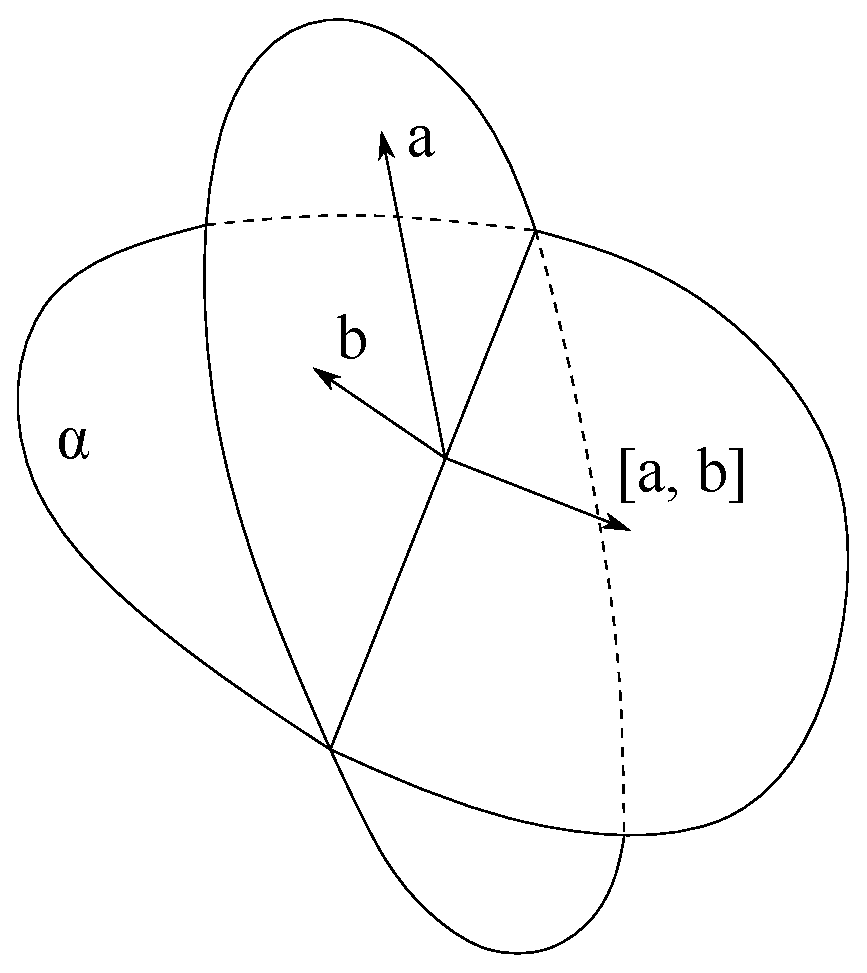
\includegraphics[width=0.5\columnwidth]{awkward-atom-or-a-pair-of-eggs}
      
      \caption{$\alpha$~---~плоскость, где лежат $[\bds a, \bds b]$, $[\bds b, \bds c]$ и $[\bds c, \bds a]$.}
      \label{fig:awkward-atom-or-a-pair-of-eggs}
    \end{figure}
    
    Рассмотрим пару векторов $\bds a$ и $\bds b$.
    Их векторное произведение $[\bds a, \bds b]$ лежит в $\alpha$ и перпендикулярно плоскости, где лежат $\bds a$ и $\bds b$ (пока считаем, что векторы $\bds a$, $\bds b$, $\bds c$ неколлинеарны).
    Таким образом, векторы $\bds a$ и $\bds b$ лежат в плоскости, перпендикулярной $\alpha$.
    Аналогично и с парами векторов $\bds a$, $\bds c$ и $\bds b$, $\bds c$.
    Все три такие плоскости попарно пересекаются хотя бы по одной прямой (например, плоскости векторов $\bds a$, $\bds b$ и векторов $\bds a$, $\bds c$ пересекаются хотя бы по прямой, содержащей вектор $\bds a$: векторы $\bds a$, $\bds b$, $\bds c$ изначально отложены от одной точки).
    Таким образом, если все три описанные плоскости совпадают, то вектора $\bds a$, $\bds b$, $\bds c$ лежат в ней, а потому компланарны.
    Если же плоскости не совпадают, а пересекаются попарно по одной прямой, то все три вектора $\bds a$, $\bds b$, $\bds c$ оказываются перпендикулярными $\alpha$, а потому параллельными.
    То есть в этом случае векторы $\bds a$, $\bds b$, $\bds c$ не только компланарны, но и коллинеарны.
    Но в процессе решения было сделано предположение о том, что $\bds a$, $\bds b$, $\bds c$ неколлинеарны, поэтому такой случай отпадает.
    
    Пусть теперь хотя бы один вектор из тройки $[\bds a, \bds b]$, $[\bds b, \bds c]$, $[\bds c, \bds a]$ равен нулевому вектору.
    Тогда либо хотя бы два вектора из трёх $\bds a$, $\bds b$, $\bds c$ коллинеарны, а потому все три они компланарны.
    Либо хотя бы один вектор из трёх $\bds a$, $\bds b$, $\bds c$ равен нулевому вектору, а потому все три снова компланарны.
  
    \bigskip
    
    \emph{``Формульный''.}
    
    Рассмотрим линейную комбинацию
    \[
      \alpha \bds a + \beta \bds b + \gamma \bds c = \bds 0
    \]
    
    Умножим векторно обе части на $\bds a$ слева.
    Получим
    \[
      \beta \cdot [\bds a, \bds b] + \gamma \cdot [\bds a, \bds c] = \bds 0
    \]
    
    Аналогично, при умножении векторно слева обеих частей исходного уравнения на $\bds b$ и $\bds c$:
    \[
      \left\{
        \begin{aligned}
          &\alpha \cdot [\bds b, \bds a] + \gamma \cdot [\bds b, \bds c] = \bds 0\\
          &\alpha \cdot [\bds c, \bds a] + \beta \cdot [\bds c, \bds b] = \bds 0
        \end{aligned}
      \right.
    \]
    
    Складывая все три полученных уравнения, получаем
    \[
      (\beta - \alpha) \cdot [\bds a, \bds b] + (\gamma - \beta) \cdot [\bds b, \bds c] + (\gamma - \alpha) \cdot [\bds a, \bds c] = \bds 0
    \]
    
    Так как векторы $[\bds a, \bds b]$, $[\bds b, \bds c]$, $[\bds c, \bds a]$ линейно зависимы, то хотя бы один из коэффициентов $(\beta \hm- \alpha)$, $(\gamma \hm- \beta)$, $(\gamma \hm- \alpha)$ может быть отличен от нуля.
    Но в таком случае три коэффициента в исходном уравнении $\alpha$, $\beta$, $\gamma$ не совпадают, а потому все три не могут в данном случае быть равны нулю одновременно.
    То есть существует нетривиальная линейная комбинация $\alpha \bds a \hm+ \beta \bds b \hm+ \gamma \bds c$, равная нулевому вектору.
    Поэтому три вектора $\bds a$, $\bds b$, $\bds c$ компланарны.
  \end{solution}
  
  
  \begin{problem}[3.27]
    Доказать, что проекция $\bds b_{\perp}$ вектора $\bds b$ на плоскость, перпендикулярную вектору $\bds a$, равна
    \[
      \bds b_{\perp} = \frac{\bigl[\bds a, [\bds b, \bds a]\bigr]}{|\bds a|^2}
    \]
  \end{problem}
  
  \begin{solution}
    Пусть $\bds b_{\parallel}$~---~составляющая вектора $\bds b$, параллельная вектору $\bds a$.
    Тогда
    \[
      \bds b = \bds b_{\parallel} + \bds b_{\perp}
    \]
    \[
      \bds b_{\perp} = \bds b - \bds b_{\parallel}
      = \bds b - \frac{(\bds b, \bds a)}{|\bds a|^2} \bds a
      = \frac{|\bds a|^2 \bds b - (\bds a, \bds b) \bds a}{|\bds a|^2}
      \xrightarrow{\mbox{``бац минус цаб''}} \frac{\bigl[\bds a, [\bds b, \bds a]\bigr]}{|\bds a|^2}
    \]
  \end{solution}
  
  
  \begin{problem}[3.33$^*$]
    Доказать, что площадь треугольника, составленного из медиан треугольника $ABC$, равна $3/4$ площади самого треугольника $ABC$.
  \end{problem}
  
  \begin{solution}
    \begin{figure}[h]
      \centering
      
      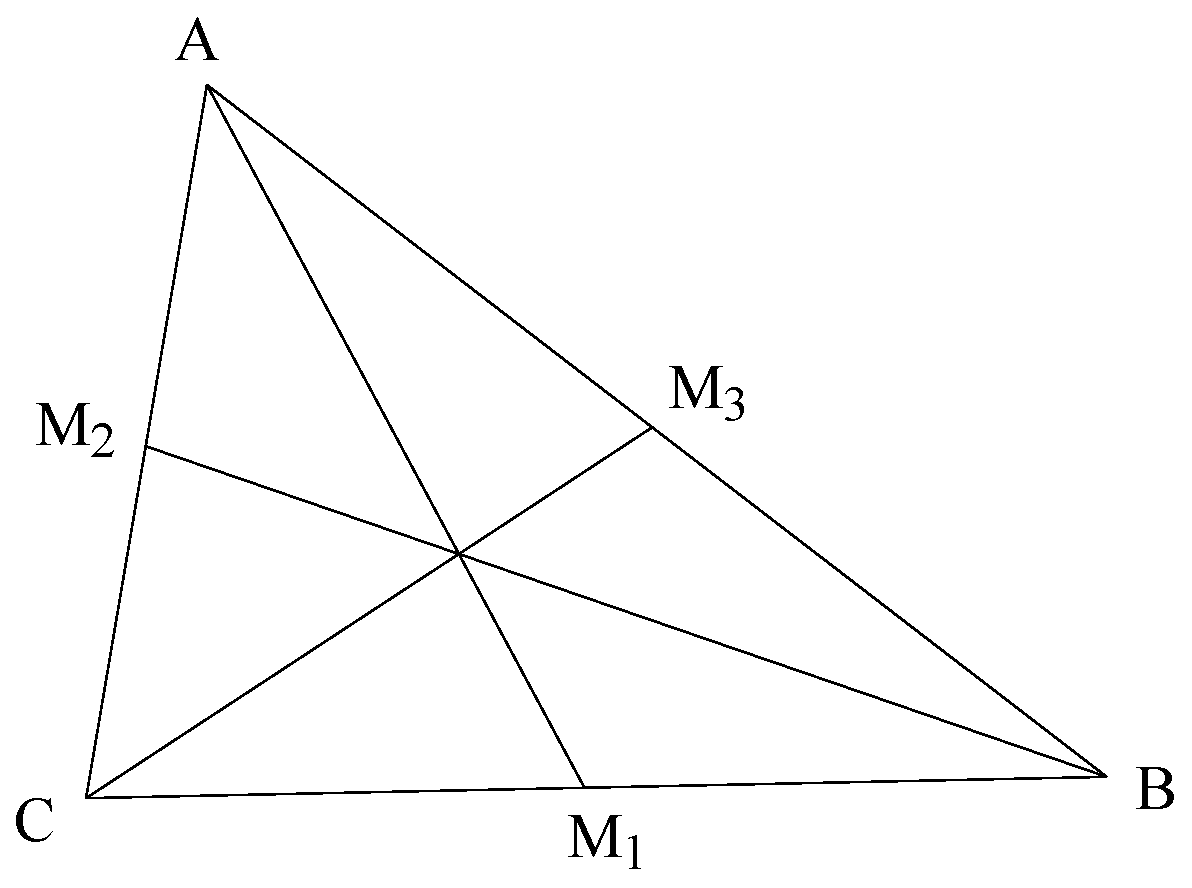
\includegraphics[width=0.5\columnwidth]{abc-m1m2m3}
      
      \caption{Медианы $AM_1$, $BM_2$ и $CM_3$ в $\triangle ABC$.}
      \label{fig:abc-m1m2m3}
    \end{figure}
    
    Пусть в треугольнике $ABC$ проведены медианы $A M_1$, $B M_2$, $C M_3$ (\ref{fig:abc-m1m2m3}).
    Проверим сначала, что из медиан в самом деле можно составить треугольник:
    \[
      \vv{AM_1} + \vv{BM_2} + \vv{CM_3} \stackrel{\?}{=} \bds 0
    \]
    
    Выразим векторы медиан через векторы сторон треугольника $ABC$:
    \[
      \left\{
        \begin{aligned}
          &\vv{AM_1} = \frac{1}{2}(\vv{AB} + \vv{AC})\\
          &\vv{BM_2} = \frac{1}{2}(\vv{BC} + \vv{BA})\\
          &\vv{CM_3} = \frac{1}{2}(\vv{CB} + \vv{CA})
        \end{aligned}
      \right.
    \]
    
    Складывая левые и правые части равенств, получаем
    \[
      \vv{AM_1} + \vv{BM_2} + \vv{CM_3} = (\vv{AB} + \vv{BA}) + (\vv{AC} + \vv{CA}) + (\vv{BC} + \vv{CB})
      = \bds 0 + \bds 0 + \bds 0 = \bds 0
    \]
    
    Теперь найдём площадь $S'$ треугольника, образованного медианами (за $S$ обозначим площадь треугольника $ABC$):
    \begin{equation*}
    \begin{split}
      S' &= \frac{1}{2} \bigl|[\vv{AM_1}, \vv{BM_2}]\bigr|
      = \frac{1}{2} \left|\left[\frac{1}{2}(\vv{AB} + \vv{AC}), \frac{1}{2}(\vv{BC} + \vv{BA})\right]\right|\\
      &= \frac{1}{8} \left|\vv{AB} \times \vv{BC} + \vv{AB} \times \vv{BA} + \vv{AC} \times \vv{BC} + \vv{AC} \times \vv{BA}\right|
      = \frac{1}{8} \cdot 3 \cdot 2 S
      = \frac{3}{4} S
    \end{split}
    \end{equation*}
    так как $\vv{AB} \hm\times \vv{BC}$, $\vv{AC} \hm\times \vv{BC}$, $\vv{AC} \hm\times \vv{BA}$ сонаправлены и по модулю равны удвоенной площади треугольника $ABC$, а $\vv{AB} \hm\times \vv{BA} \hm= \bds 0$.
  \end{solution}
  
  
  \begin{problem}[3.31]
    Решить систему векторных уравнений в пространстве
    \[
      \left\{
        \begin{aligned}
          (\bds x, \bds a) = p\\
          (\bds x, \bds b) = q\\
          (\bds x, \bds c) = s
        \end{aligned}
      \right.
    \]
    где векторы $\bds a$, $\bds b$ и $\bds c$ некомпланарны.
  \end{problem}
  
  \begin{solution}
    Сначала покажем, что если $\bds a$, $\bds b$ и $\bds c$ некомпланарны, то и $[\bds a, \bds b]$, $[\bds b, \bds c]$ и $[\bds a, \bds c]$ некомпланарны.
    Рассмотрим линейную комбинацию
    \[
      \alpha [\bds a, \bds b] + \beta [\bds b, \bds c] + \gamma [\bds c, \bds a] = \bds 0
    \]
    Умножим обе части скалярно на $\bds b$ слева.
    Получим
    \[
      \gamma (\bds b, \bds c, \bds a) = \bds 0
    \]
    Откуда $\gamma \hm= 0$, так как $\bds a$, $\bds b$ и $\bds c$ некомпланарны (и их смешанное произведение отлично от нуля).
    Аналогично $\alpha \hm= 0$ и $\beta \hm= 0$.
    Поэтому три вектора $[\bds a, \bds b]$, $[\bds b, \bds c]$ и $[\bds a, \bds c]$ также некомпланарны.
    
    \bigskip
    
    Введём понятие \emph{взаимного базиса}.
    
    \begin{definition}
      Пусть есть базис $e \hm= (\bds e_1, \bds e_2, \bds e_3)$.
      Тогда взаимный базис $e^* \hm= (\bds e_1^*, \bds e_2^*, \bds e_3^*)$ определяется как
      \begin{equation}\label{eq:dual-basis}
        \left\{
          \begin{aligned}
            &\bds e_1^* = \frac{[\bds e_2, \bds e_3]}{(\bds e_1, \bds e_2, \bds e_3)}\\
            &\bds e_2^* = \frac{[\bds e_3, \bds e_1]}{(\bds e_1, \bds e_2, \bds e_3)}\\
            &\bds e_3^* = \frac{[\bds e_1, \bds e_2]}{(\bds e_1, \bds e_2, \bds e_3)}
          \end{aligned}
        \right.
      \end{equation}
    \end{definition}
    
    По доказанному ранее, $e^*$ в самом деле базис (три линейно независимых вектора в пространстве).
    Также можно заметить, что $(\bds e_i, \bds e_i^*) \hm= 1$ и $(\bds e_i, \bds e_j^*) \hm= 0$ при $i \hm{\not=} j$ (поэтому базис $e^*$ также называют биортогональным к базису $e$)\footnote{Эти свойства на самом деле определяют взаимный базис в общем случае $\RR^n$ (\href{https://en.wikipedia.org/wiki/Dual\_basis}{en.wikipedia.org/wiki/Dual\_basis}).}.
    
    \bigskip
    
    Возвращаясь к задаче, разложим вектор $\bds x$ по взаимному к $\{\bds a, \bds b, \bds c\}$ базису $\{\bds a^*, \bds b^*, \bds c^*\}$:
    \[
      \bds x = x_1^* \bds a^* + x_2^* \bds b^* + x_3^* \bds c^*
    \]
    
    Умножая скалярно по очереди на $\bds a$, $\bds b$, $\bds c$ и пользуясь свойством ``биортогональности'' взаимного базиса, получаем
    \[
      \left\{
        \begin{aligned}
          &(\bds x, \bds a) = x_1^*\\
          &(\bds x, \bds b) = x_2^*\\
          &(\bds x, \bds c) = x_3^*
        \end{aligned}
      \right.
    \]
    
    То есть числа $p$, $q$ и $s$, данные в условии, есть компоненты вектора $\bds x$ во взаимном к $\{\bds a, \bds b, \bds c\}$ базисе, векторы которого вычисляются по (\ref{eq:dual-basis}).
  \end{solution}
  
  
  \begin{problem}[3.22(1)]
    Три некомпланарных вектора $\bds a$, $\bds b$, $\bds c$ отложены из одной точки.
    Найти объём треугольной призмы, основание которой построено на $\bds a$ и $\bds b$, а боковое ребро совпадает с вектором $\bds c$.
  \end{problem}
  
  \begin{solution}
    \begin{figure}[h]
      \centering
      
      \includegraphics[width=0.5\columnwidth]{triangular-prism}
      
      \caption{Треугольная призма, построенная на $\bds a$, $\bds b$ и $\bds c$.}
      \label{fig:triangular-prism}
    \end{figure}
    
    Объём призмы $V'$ равен произведению площади основания на высоту (\ref{fig:triangular-prism}).
    В основании треугольник~---~площадь которого в два раза меньше площади параллелограмма, построенного на тех же векторах $\bds a$ и $\bds b$.
    То есть объём призмы ищется аналогично объёму $V$ параллелепипеда, построенного на $\bds a$, $\bds b$, $\bds c$, только площадь основания в два раза меньше.
    Поэтому и
    \[
      V' = \frac{1}{2} V = \frac{\bigl|(\bds a, \bds b, \bds c)\bigr|}{2}
    \]
    
    Задача решена.
    Нашли объём, не находя ни высоты, ни площади основания.
    
    \bigskip
    
    \emph{Отступление.}
    
    Но как можно бы было найти вектор $\bds c_{\perp}$, по модулю равный высоте призмы и перпендикулярный основаниям?
    Вектор $\bds c$ можно представить в виде суммы двух векторов, один из которых параллелен плоскости основания призмы, а другой перпендикулярен плоскости основания.
    В свою очередь, компоненту $\bds c$, параллельную основаниям, можно разложить по векторам $\bds a$ и $\bds b$ (которые, как неколлинеарные вектора, образуют базис на плоскости).
    Получаем
    \[
      \bds c = \alpha \bds a + \beta \bds b + \bds c_{\perp}
    \]

    Если умножить полученное уравнение скалярно на $\bds a$ и на $\bds b$ (по очереди), то получим систему
    \[
      \left\{
        \begin{aligned}
          &(\bds c, \bds a) = \alpha (\bds a, \bds a) + \beta (\bds b, \bds a)\\
          &(\bds c, \bds b) = \alpha (\bds a, \bds b) + \beta (\bds b, \bds b)
        \end{aligned}
      \right.
    \]
    из которой уже можно найти $\alpha$ и $\beta$, например, по правилу Крамера, если определитель системы отличен от нуля:
    \[
      \Delta = \begin{vmatrix}
        (\bds a, \bds a) & (\bds a, \bds b)\\
        (\bds a, \bds b) & (\bds b, \bds b)
      \end{vmatrix}
      = |\bds a|^2 |\bds b|^2 - |\bds a|^2 |\bds b|^2 \cos^2 \angle{(\bds a, \bds b)}
      = \bigl|[\bds a, \bds b]\bigr|^2
      \not= 0
    \]
    так как векторы $\bds a$ и $\bds b$ неколлинеарны.
    А вообще, определитель
    \[
      \begin{vmatrix}
        (\bds a, \bds a) & (\bds a, \bds b)\\
        (\bds a, \bds b) & (\bds b, \bds b)
      \end{vmatrix}
    \]
    называется \emph{определителем Грама\footnote{\href{https://en.wikipedia.org/wiki/Gramian\_matrix}{en.wikipedia.org/wiki/Gramian\_matrix}.}} системы векторов $\bds a$ и $\bds b$.
    Из решения видно, что отличие от нуля определителя Грама системы векторов является \emph{критерием линейной независимости} этой системы векторов (чтобы коэффициенты разложения любого вектора по этой системе определялись однозначно~---~в нашем случае коэффициенты разложения компоненты $\bds c$, параллельной основанию призмы, по векторам $\bds a$ и $\bds b$).
    
    Возвращаясь к вектору $\bds c_{\perp}$, то при найденных $\alpha$ и $\beta$ он получается равным
    \[
      \bds c_{\perp} = \bds c - \alpha \bds a - \beta \bds b
    \]
  \end{solution}
\end{document}
